\section{习题参考答案}
\subsection*{一、填空题}
\begin{enumerate}
    \item 如图~\ref{Fig:65},一个带电$Q$的粒子($Q>0$),以速度$V$向右运动,求距粒子$r$处产生的磁感应强度为$B$=\anl{$\frac{\mu_0}{4\pi}\cdot\frac{QV}{r^2}$},方向为\anl{垂直纸面向里
    }.
    \begin{figure}[H]
        \centering
        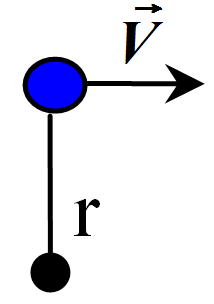
\includegraphics[width=0.25\textwidth]{fig65}
        \caption{如图所示}\label{Fig:65}
    \end{figure}
    \item 一个无限长的圆形螺线管,单位长度匝数为$n$,通有电流强度$I$,则在螺线管内部的磁感应强度大小$B$=\anl{$\mu_0 mI$}.
    \begin{note}
        \textcolor{red}{无限长螺线管产生磁场:$B=\mu_0 n I$}
    \end{note}
    \item 如图~\ref{Fig:66},一平面线圈由半径为~$R$~的1/4圆弧和相互垂直的二直线组成,通以电流$I$,把它放在磁感强度为~$B$~的均匀磁场中,则线圈磁矩大小$p_m$=\anl{$\frac{1}{4}I\pi R^2$}.
    \begin{figure}[H]
        \centering
        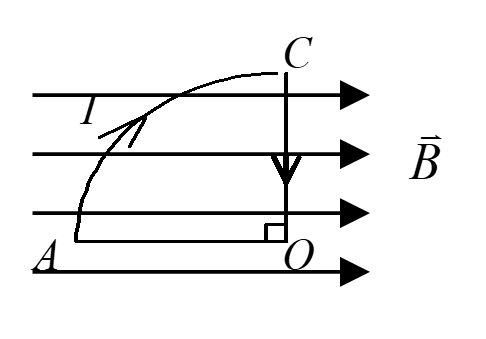
\includegraphics[width=0.25\textwidth]{fig66}
        \caption{如图所示}\label{Fig:66}
    \end{figure}
    \begin{note}
        \textcolor{red}{$\vec{p}_m=IS\vec{n}, p_m=IS=I\cdot \frac{1}{4}\pi R^2$.}
    \end{note}
    \item 如图~\ref{Fig:67}, 真空中环绕两根通有电流为$I$的导线的两种环路,则对环路$L_1$有$\oint_{l1}\vec{B}\cdot \mathrm{d}\vec{l}$=\anl{0},对环路$L_2$有$\oint_{l2}\vec{B}\cdot \mathrm{d}\vec{l}$=\anl{$2\mu_0 I$}.
    \begin{figure}[H]
        \centering
        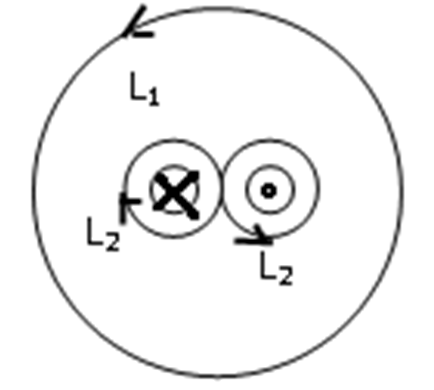
\includegraphics[width=0.25\textwidth]{fig67}
        \caption{如图所示}\label{Fig:67}
    \end{figure}
    \begin{note}
        \textcolor{red}{$\oint_L \vec{B}\cdot \dd \vec{L}=\mu_0 \sum I_i$, $L_1$内包含的电流:0 ; $L_2$内包含的电流:$2I$.}
    \end{note}
    \item 在安培环路定理$\oint_{l} \vec{B}\cdot \mathrm{d}\vec{l}$中, $\sum \mathbf{I_i}$是指\underline{闭合路径$L$所包围的电流强度的代数和};$\vec{B}$~是指\underline{闭合路径$L$上各点的磁感应强度};它是由\underline{全空间所有电流} 决定的.
    \item 一半径为$a$的无限长直载流导线,沿轴向均匀地流有电流$I$,若作一个半径为$R=5a$,高为$L$的柱形曲面,已知柱形曲面的轴与载流导线的轴平行且相距$3a$,如图~\ref{Fig:68},则$B$在圆柱侧面$S$上的积分~$\int_S \vec{B}\cdot \mathrm{d} \vec{S}$=\underline{0}.
    \begin{figure}[H]
        \centering
        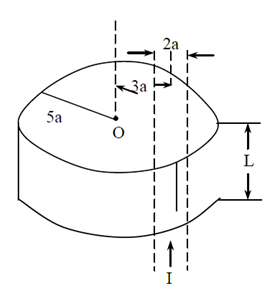
\includegraphics[width=0.25\textwidth]{fig68}
        \caption{如图所示}\label{Fig:68}
    \end{figure}
    \begin{note}
        \textcolor{red}{$\oint_S \vec{B}\cdot \dd \vec{S}=0$}
    \end{note}
    \item 通有电流$I$ 的长直导线在一平面内被弯成如图~\ref{Fig:69}~形状($R$为已知),放于垂直进入纸面的均匀磁场$\vec{B}$中,则整个导线所受的安培力大小$F$=\anl{$2IBR$}.
     \begin{figure}[H]
        \centering
        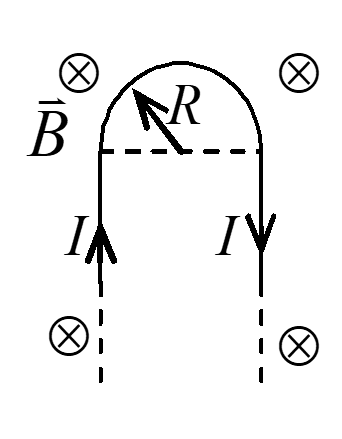
\includegraphics[width=0.25\textwidth]{fig69}
        \caption{如图所示}\label{Fig:69}
    \end{figure} 
    \begin{note}
        \textcolor{red}{具体如下:}
        \begin{figure}[H]
            \centering
            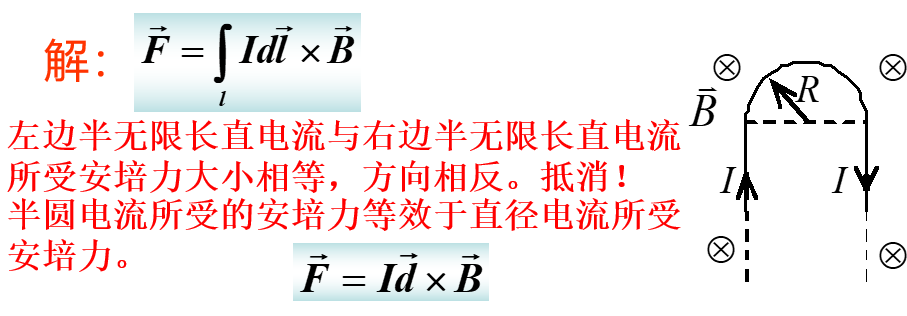
\includegraphics[width=0.35\textheight]{ans49}
        \end{figure}
    \end{note}
    \item 如图所示~\ref{Fig:70},平行放置在同一平面内的三条载流长直导线,电流依次是$I$,$I$,$2I$要使导线$AB$所受的安培力等于零,则
    $x$=\anl{$a/3$}.
    \begin{figure}[H]
        \centering
        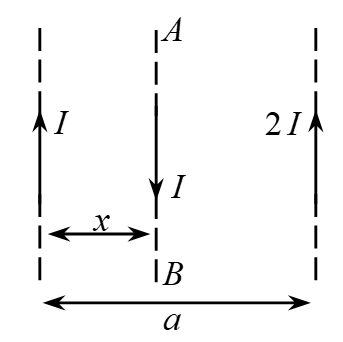
\includegraphics[width=0.25\textwidth]{fig70}
        \caption{如图所示}\label{Fig:70}
    \end{figure}
    \begin{note}
        \textcolor{red}{具体如下:}
        \begin{figure}[H]
            \centering
            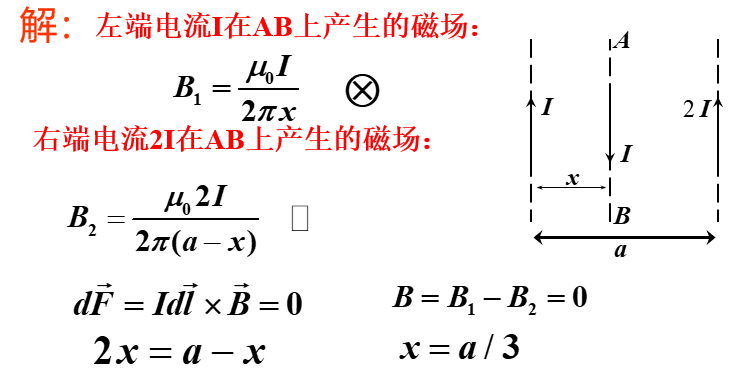
\includegraphics[width=0.35\textheight]{ans50}
        \end{figure}
    \end{note}
\end{enumerate}
\subsection*{二、选择题}
\begin{enumerate}
    \item 长直导线通有电流$I$,将其弯成如图所示\ref{Fig:71}形状,则$O$点处的磁感应强度大小为~\anss{B}
    \twoch{$\frac{\mu_0I}{2\pi R}+\frac{\mu_0 I}{4R}$}{$\frac{\mu_0 I}{4\pi R}+\frac{\mu_0 I}{8R}$}{$\frac{\mu_0 I}{2\pi R}+\frac{\mu_0 I}{8 R}$}{$\frac{\mu_0 I}{4\pi R}+\frac{\mu_0 I}{4 R}$}
    \insertfig{0.25}{fig71}{Fig:71}
    \begin{note}
        \textcolor{red}{具体如下:}
        \begin{figure}[H]
            \centering
            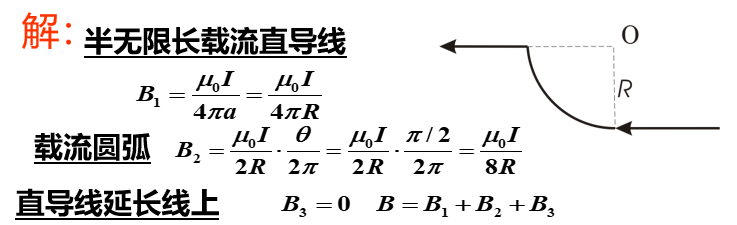
\includegraphics[width=0.35\textheight]{ans51}
        \end{figure}
    \end{note}
    \item 一根载有电流$I$的无限长直导线,在$A$处弯成半径为$R$的圆形,由于导线外有绝缘层,在$A$处两导线并不短路,则在圆心处磁感应强度$\vec{B}$的大小为~\anss{C}
    \twoch{$I(\mu_0 +1 )/(2\pi R)$}{$\mu_0 \pi I / (2\pi R)$}{$\mu I (1+\pi R)$}{$\mu_0 I (1+\pi)/(4\pi R)$}
    \begin{note}
        \textcolor{red}{具体如下:}
        \begin{figure}[H]
            \centering
            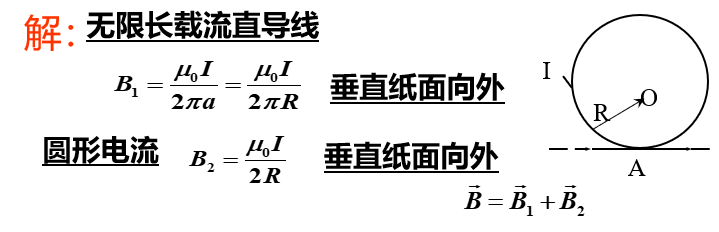
\includegraphics[width=0.35\textheight]{ans52}
        \end{figure}
    \end{note}
    \item 四条相互平行的载流长直导线电流强度均为$I$,方向如图\ref{Fig:73}。设正方形的边长为$2a$,则正方形中心的磁感应强度为~\anss{D}
    \fourch{$\frac{2\mu_0}{\pi a}I$}{$\frac{2\mu_0}{\sqrt{2}\pi a}I$}{$\frac{\mu_0}{\pi a}I$}{$0$}
    \insertfig{0.25}{fig72}{Fig:72}
    \begin{note}
        \textcolor{red}{正方形对角的两无限长直线电流在其中心产生的磁感应强度大小相等,方向相反,互相抵消。}
    \end{note}
    \item 如图\ref{Fig:73}, 在磁感强度为$\vec{B}$的均匀磁场中作一半径为$r$的半球面$S$,$S$边线所在平面的法线方向单位矢量$\vec{n}$与$\vec{B}$的夹角为$\alpha$,则通过半球面$S$的磁通量(取弯面向外为正)为~\anss{D}
    \fourch{$\pi r^2 B$}{$2\pi r^2 B$}{$-\pi r^2 B \mathrm{sin} \alpha$}{$-\pi r^2 B\mathrm{cos}\alpha$}
    \insertfig{0.25}{fig73}{Fig:73}
    \begin{note}
        \textcolor{red}{下底面的磁通量: $\varPhi_2=\vec{B}\cdot \vec{S}=\pi r^2 B \mathrm{cos} \alpha$; 通过半球面$S$的磁通量:$\varPhi_1=-\varPhi_2=-\pi r^2 B \mathrm{cos}\alpha$}
    \end{note}
    \item 如图\ref{Fig:74},两根直导线~$ab$~和~$cd$~沿半径方向被接到一个截面处处相等的铁环上,稳恒电流$I$从$a$端流入而从$d$端流出,则磁感强度$\vec{B}$沿图中包围铁环截面的闭合路径$L$的积分$\oint_L \vec{B}\cdot \dd \vec{l}$等于~\anss{D}
    \fourch{$\mu_0I$}{$-\mu_0 I/3$}{$2\mu_0I/3$}{$-2\mu_0 I/3$}
    \insertfig{0.25}{fig74}{Fig:74}
    \begin{note}
        \textcolor{red}{$R=\rho\frac{l}{S}$, $R_{240^\circ}=2R_{120^\circ}$, $I_{120^\circ}=2I_{240^\circ}=2I/3$与$L$规定的正向相反。$\therefore \oint_S\vec{B}\cdot \dd \vec{L}=\mu_0 \sum I_i=-2\mu_0 I /3$}
    \end{note}
    \item 如图所示\ref{Fig:75},流出纸面的电流为$2I$,流进纸面的电流为$I$,则下述式中哪一个是正确的是~\anss{D}
    \twoch{$\oint_{L1}\vec{B}\cdot \dd \vec{l}=2\mu_0 I$}{$\oint_{L2}\vec{B}\cdot \dd \vec{l}=\mu_0 I$}{$\oint_{L3}\vec{B}\cdot \dd \vec{l}=-\mu_0 I$}{$\oint_{L4}\vec{B}\cdot \dd \vec{l}=-\mu_0 I$}
    \insertfig{0.25}{fig75}{Fig:75}
    \begin{note}
        \textcolor{red}{$\oint_L \vec{B}\cdot \dd \vec{L}=\mu_0 \sum I_i$, 符号规定:电流方向与$L$的环绕方向服从右手关系的$I$为正,否则为负。}
    \end{note}
    \item 如图~\ref{Fig:76}~六根互相绝缘导线,通以电流强度均为$I$,区域$I$、$II$、$III$、$IV$均为正方形,那么指向纸内的磁通量最大的区域是~\anss{B}
    \fourch{$I$区域}{$II$区域}{$III$区域}{$IV$区域}
    \insertfig{0.25}{fig76}{Fig:76}
    \begin{note}
        \textcolor{red}{右手螺旋法则:左边两竖直电流在II、IV区域磁场向纸内;下面两水平电流在I、II区域磁场向纸内; }
    \end{note}
    \item 无限长直导线通有电流$I$,右侧有两个相连的矩形回路,分别是$S_1$和$S_2$,则通过两个矩形回路$S_1$、$S_2$的磁通量之比为~\anss{B}
    \fourch{1:2}{1:1}{1:4}{2:1}
    \insertfig{0.25}{fig77}{Fig:77}
    \begin{note}
        \textcolor{red}{具体如下:}
        \begin{figure}[H]
            \centering
            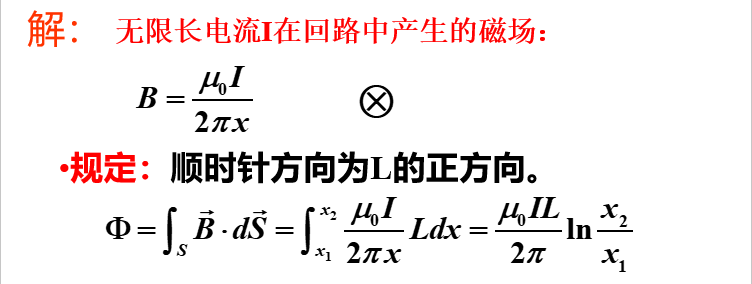
\includegraphics[width=0.35\textheight]{ans53}
        \end{figure}
    \end{note}
\end{enumerate}
\subsection*{三、计算题}
\begin{enumerate}
    \item 载有电流为$I$的无限长导线,弯成如图~\ref{Fig:78}~形状,其中一段是半径为$a$的半圆,求圆心处的磁感应强度$\vec{B}$的大小.
    \insertfig{0.25}{fig78}{Fig:78}
    \begin{solution}
        如图:
        \begin{figure}[H]
            \centering
            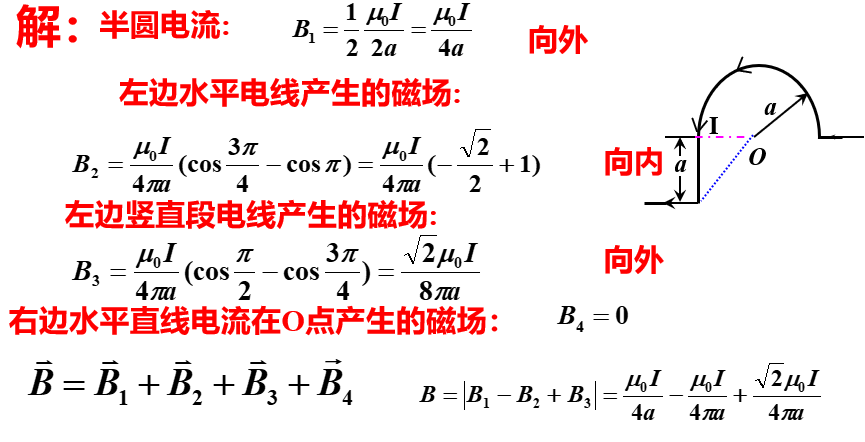
\includegraphics[width=0.55\textheight]{ans54}
        \end{figure}
    \end{solution}
    \item 如图~\ref{Fig:79}~半径为$R$的带电圆盘,电荷面密度为$\sigma$,圆盘以角速度$\omega$绕过盘心并垂直盘面的轴旋转,求中心$O$处的磁感应强度$\vec{B}$。
    \insertfig{0.25}{fig79}{Fig:79}
    \begin{solution}
        如图:
        \begin{figure}[H]
            \centering
            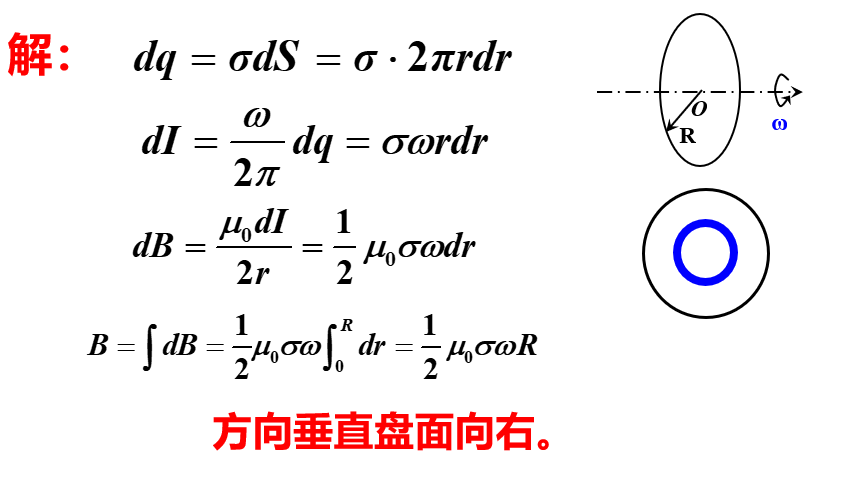
\includegraphics[width=0.35\textheight]{ans55}
        \end{figure}
    \end{solution}
    \item 如图~\ref{Fig:80}一半径为$R$的无限长圆柱形导体,现有电流$I$均匀地流过导体横截面,且电流方向与导体轴线平行,求空间的磁场分布。
    \insertfig{0.25}{fig80}{Fig:80}
    \begin{solution}
        如图:
        \begin{figure}[H]
            \centering
            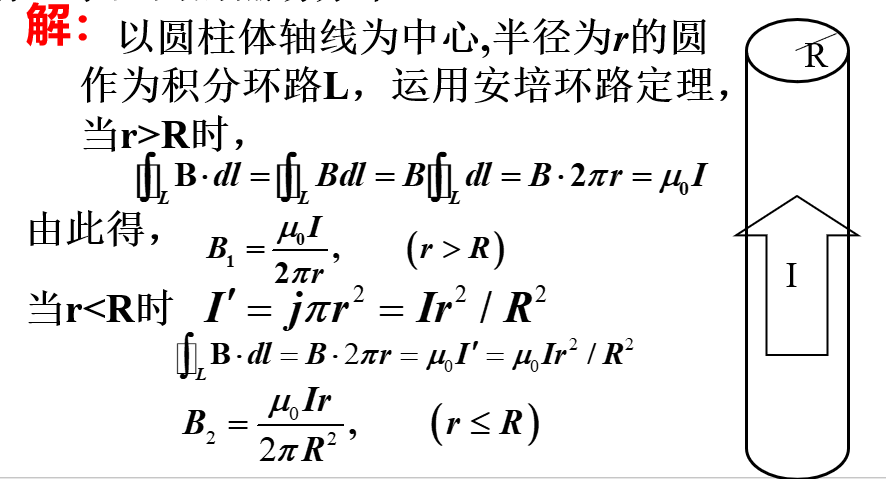
\includegraphics[width=0.55\textheight]{ans56}
        \end{figure}
    \end{solution}
    \item 如图~\ref{Fig:81}~在载流为$I_1$的长直导线旁,共面放置一载流为$I_2$的等腰直角三角形线圈$abc$,腰长$ab=ac=L$,边长$ab$平行于长直导线,相距$L$,求线圈各边受的磁力$F$.
    \insertfig{0.25}{fig81}{Fig:81}
    \begin{solution}
        如图:
        \begin{figure}[H]
            \centering
            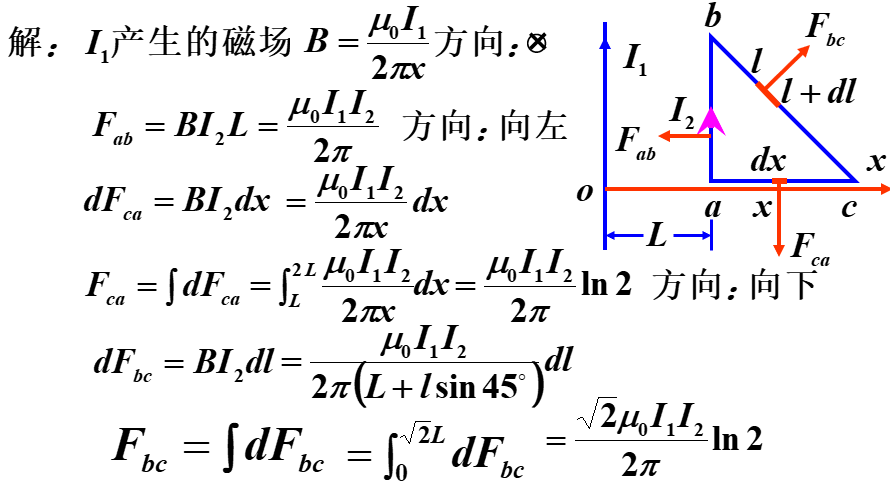
\includegraphics[width=0.55\textheight]{ans57}
        \end{figure}
    \end{solution}
    \item 如图~\ref{Fig:82}无限长直导线和半径为$R$的圆形线圈,彼此绝缘,共面放置,且圆线圈直径和直导线重合,直导线与圆线圈分别通以电流$I_1$和$I_2$,求
    \begin{enumerate}[label=(\arabic*)]
        \item 长直导线对半圆弧$abc$所作用的磁力;
        \item 整个圆形线圈所受的磁力.
    \end{enumerate}
    \insertfig{0.25}{fig82}{Fig:82}
    \begin{solution}
        如图:
        \begin{figure}[H]
            \centering
            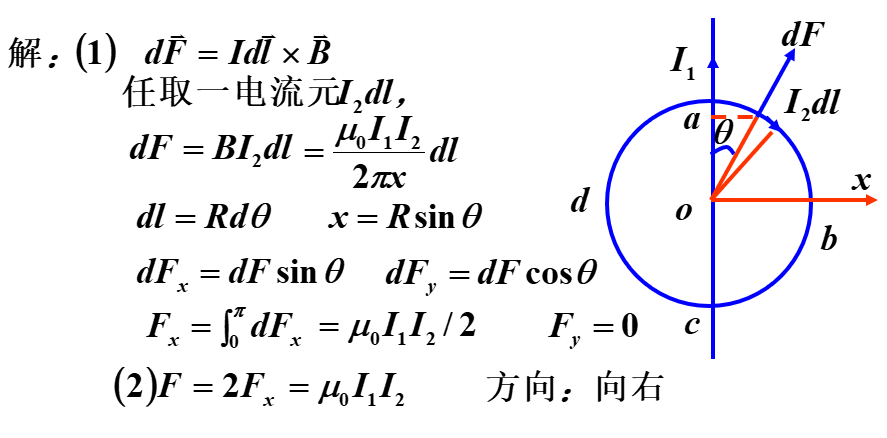
\includegraphics[width=0.55\textheight]{ans58}
        \end{figure}
    \end{solution}
\end{enumerate}